\documentclass[11pt,a4paper]{article}

\usepackage[margin=2cm]{geometry}
\usepackage{amsmath,amssymb}
\usepackage{graphicx}
\usepackage{caption}
\usepackage{subcaption}
\usepackage{booktabs}
\usepackage{tabularx}
\usepackage{array}
\usepackage{longtable}
\usepackage[table]{xcolor}
\usepackage{listings}
\usepackage{enumitem}
\usepackage[hidelinks]{hyperref}

\graphicspath{{figures/}}

% basis of each setting
\definecolor{notstated}{RGB}{235,235,235}
\definecolor{changed}{RGB}{255,228,196}
\newcommand{\Nrow}{\rowcolor{notstated}}
\newcommand{\Crow}{\rowcolor{changed}}

\newcolumntype{L}[1]{>{\raggedright\arraybackslash}p{#1}}
\newcolumntype{Y}{>{\raggedright\arraybackslash}X}

\lstset{
  language=Matlab,
  basicstyle=\ttfamily\scriptsize,
  commentstyle=\color{black!55},
  keywordstyle=\color{blue!60!black},
  columns=fullflexible,
  keepspaces=true,
  frame=single,
  framerule=0.3pt,
  breaklines=true,
  showstringspaces=false,
  aboveskip=4pt,
  belowskip=4pt
}

\newcommand{\file}[1]{\texttt{#1}}
\newcommand{\E}{\mathbb{E}}
\newcommand{\QA}[2]{\item \textbf{Q: #1}\\ \textbf{A:} #2}
\renewcommand{\arraystretch}{1.15}

\begin{document}

\begin{center}
{\Large\bfseries Simulation Reference Notes\\[2pt]
Reproduction of Figs.~3--5 of\\[2pt]
``Channel Estimation for Rydberg Atomic Receivers''}\\[6pt]
{\normalsize What was simulated, which values were used, why, and how to defend them}
\end{center}

\vspace{0.5em}

\section{What this document is}

These are my own reference notes for the MATLAB reproduction of Figs.~3--5 of
Xu \emph{et al.}~\cite{xu2025}. They record, for every figure:
\begin{itemize}[leftmargin=*,itemsep=1pt]
  \item which values the paper gives and which it does not give;
  \item which value I used for every setting the paper does not give, and why;
  \item what is different between the \textbf{literal} and the \textbf{tuned} script;
  \item what the results are, what matches the paper and what cannot match;
  \item the questions my guide may ask, with the answers.
\end{itemize}
Equation numbers refer to~\cite{xu2025} unless stated otherwise. Reference~\cite{cui2024} is the
paper from which Xu \emph{et al.} take the biased Gerchberg--Saxton (GS) method.

\subsection{Files}

Each script writes a figure (\file{.png}) and a results file (\file{.mat}) with the same name as
the script. All scripts use \file{rng(1)}, so every run gives the same numbers.

\begin{table}[h]
\centering
\small
\caption{Simulation scripts (folder \file{Channel\_Estimation\_for\_Rydberg\_Atomic\_Receivers/}).}
\label{tab:files}
\begin{tabularx}{\textwidth}{L{3.6cm} L{5.2cm} Y}
\toprule
Figure & Script & Purpose \\
\midrule
Fig.~3 (1D, NMSE vs SNR) & \file{fig3/fig3\_literal/fig3\_literal.m} & only the values stated in the paper \\
                         & \file{fig3/fig3\_tuned/fig3\_tuned.m} & same equations, settings chosen to reproduce the published figure \\
                         & \file{fig3/fig3\_converged/fig3\_converged.m} & same as tuned, but GS and GD run to convergence (fair comparison) \\
Fig.~4 (2D, NMSE vs SNR) & \file{fig4/fig4\_literal/fig4\_literal.m} & only the values stated in the paper \\
                         & \file{fig4/fig4\_tuned/fig4\_tuned.m} & tuned \\
Fig.~5 (2D, NMSE vs $P$) & \file{fig5/fig5\_literal/fig5\_literal.m} & only the values stated in the paper \\
                         & \file{fig5/fig5\_tuned/fig5\_tuned.m} & tuned \\
\bottomrule
\end{tabularx}
\end{table}

\subsection{Literal and tuned in one paragraph}

The \textbf{literal} scripts use every value exactly as the paper states it. They do
\emph{not} reproduce the published figures: all curves flatten near 0\,dB (Section~\ref{sec:c1}).
The \textbf{tuned} scripts use the same equations and the same algorithms. They change three
things, each marked \file{\% TUNED} in the code: the strength of the reference signal (C1), where
the polarization is drawn (C2), and the number of iterations (C3). With these three changes the
published behaviour is reproduced.

\subsection{Marks used in the tables}

\begin{center}
\small
\begin{tabular}{lll}
\toprule
Mark & Meaning & Row colour \\
\midrule
S & stated in~\cite{xu2025} (or in~\cite{cui2024} for GS) and used as stated & white \\
N & not stated in~\cite{xu2025}; I chose a value & \colorbox{notstated}{grey} \\
C & changed in the tuned scripts & \colorbox{changed}{orange} \\
\bottomrule
\end{tabular}
\end{center}

%=====================================================================
\section{What the paper gives and what it does not give}
\label{sec:given}

\begin{table}[h!]
\centering
\small
\caption{Values stated in the paper (used unchanged in the literal scripts).}
\label{tab:stated}
\begin{tabularx}{\textwidth}{L{4.2cm} Y}
\toprule
Item & Value stated in the paper \\
\midrule
Transition dipole moment & $\mu_{eg}=[0,\;1785.9\,q a_0,\;0]^T$ \\
Users, paths & $K=3$; $L_k$ uniform on $\{3,\dots,7\}$ \\
Path gains & $\alpha_{l,k}\sim\mathcal{CN}(0,1)$ \\
Reference path gain & $\alpha_b\sim\mathcal{CN}(0,10)$ \\
Polarization & components $\sim\mathcal{N}(0,1/3)$; the vectors carry a vapor-cell index ($\epsilon_{i,k,l}$, $\epsilon_{b,i}$) in Eqs.~(7), (9), (16), (17) \\
Pilots & $s_{k,p}\sim\mathcal{CN}(0,1)$ \\
Initial estimate & $G_0\sim\mathcal{CN}(0,0.1)$ \\
Array & Fig.~3: 1D, $I=8$ cells. Figs.~4--5: 2D, $8\times8$ cells \\
Pilot lengths, SNR & Figs.~3--4: $P\in\{10,30\}$, SNR $-5$ to 30\,dB. Fig.~5: $P=5$ to 50, SNR 5\,dB \\
Measurement & magnitude only, $y=|\,\text{signal}+b+n\,|$, Eq.~(8) and its 2D form \\
Estimators & GD, Eqs.~(13)--(15); PGD, Algorithm~1, Eqs.~(23)--(27), with rank $L_k$ per user (Eqs.~(21), (25)); GS from~\cite{cui2024} \\
Bound & CRLB, Eqs.~(29)--(31) \\
NMSE & $\E\{\|G-\hat G\|_F^2\}/\E\{\|G\|_F^2\}$ (Sec.~V) \\
\bottomrule
\end{tabularx}
\end{table}

\begin{table}[h!]
\centering
\small
\caption{Settings the paper does not give, the value I used, and the reason.}
\label{tab:notstated}
\begin{tabularx}{\textwidth}{L{3.0cm} L{4.6cm} Y}
\toprule
Not given in the paper & Value used (all scripts) & Reason \\
\midrule
\Nrow SNR definition & SNR $=\E|a|^2/\sigma^2$ per cell and per pilot, where $a$ are the entries of the noiseless users' signal ($GS$ in 1D, $S^TG_{(3)}$ in 2D) and $\sigma^2$ is the complex noise variance & The paper never defines SNR. This is the definition of~\cite{cui2024}, Eq.~(36), the paper from which the GS baseline is taken. \\
\Nrow Step size $\mu$ & $\mu=1/\lambda_{\max}(SS^H)$ & The paper assumes a Lipschitz-continuous gradient (Sec.~III) but gives no value. $\lambda_{\max}(SS^H)$ is the Lipschitz constant, so $1/L$ is the standard safe step. \\
\Nrow Stopping rule & stop when $\|G^{t+1}-G^{t}\|_F^2<10^{-12}\,\|G^{t+1}\|_F^2$, at most 3000 iterations (literal scripts) & Algorithm~1 stops at ``a pre-defined threshold'' but gives no value. $10^{-12}$ means ``run until converged''. \\
\Nrow GS iterations & 50 (literal) & \cite{cui2024} uses $t_0=50$. \\
\Nrow Reference pilot & $s_{b,p}=1$ for all $p$ & Not given. A constant reference is the simplest choice; a check with random $s_{b,p}\sim\mathcal{CN}(0,1)$ changed the result by at most about 1.4\,dB. \\
\Nrow Element spacing & $d=\lambda/2$ & Standard value. \\
\Nrow Angles & 1D: angle of arrival uniform on $(0,2\pi)$. 2D: elevation uniform on $(0,\pi)$, azimuth uniform on $(0,2\pi)$ & Not given. Uniform over all directions. \\
\Nrow Monte Carlo trials & 500 per point & Not given. Channel, pilots and reference are drawn once per trial and reused for every SNR. \\
\Nrow NMSE averaging & ratio of sums over all trials & Matches the definition $\E\{\cdot\}/\E\{\cdot\}$ of Sec.~V. \\
\bottomrule
\end{tabularx}
\end{table}

\paragraph{One deviation from the printed equations.}
Eqs.~(26)--(27) write the SVD reconstruction as $U\Sigma V^{T}$. For a complex matrix the correct
reconstruction is $U\Sigma V^{H}$; with $V^T$ the result is not the best rank-$L_k$ approximation.
All 2D scripts use $V^H$ (MATLAB \file{V'}).

%=====================================================================
\section{The three changes in the tuned scripts}
\label{sec:changes}

\subsection{C1: strength of the reference (RSR $=50$\,dB)}
\label{sec:c1}

\paragraph{Definition.} Reference-to-signal ratio:
$\text{RSR}=\E|b|^2/\E|a|^2$, where $b$ are the entries of the reference and $a$ the entries of the
noiseless users' signal.

\paragraph{What the paper gives.} $\alpha_b\sim\mathcal{CN}(0,10)$. Nothing else about how strong the
reference is compared with the users' signal.

\paragraph{Why it had to change.}
\begin{enumerate}[leftmargin=*,itemsep=1pt]
  \item GD and PGD are built on the linearised model of Eq.~(12),
        $|a+b|\approx|b|+\mathrm{Re}(z\,a)$. This is only accurate when $|b|\gg|a|$.
  \item With the paper's values the reference is \emph{weaker} than the signal. The literal scripts
        measure it: RSR $=-1.4$ to $-2.1$\,dB in all three figures
        (Fig.~3: $-1.5$, $-1.8$\,dB; Fig.~4: $-2.0$, $-2.1$\,dB; Fig.~5: $-1.4$ to $-2.1$\,dB).
        The users' signal is a sum over 3 users with 3--7 paths each; the reference has one path.
  \item So in the literal runs the linearisation fails and all curves flatten near 0\,dB
        (up to 34\,dB above the CRLB at 30\,dB SNR), even though the algorithms have converged.
\end{enumerate}

\paragraph{What I did.} $\alpha_b$ is still drawn from $\mathcal{CN}(0,10)$; the reference is then
scaled by one constant so that RSR $=50$\,dB in every trial:
\begin{lstlisting}
B = B*sqrt(10^(RSR_dB/10)*signalPower/mean(abs(B(:)).^2));   % RSR_dB = 50, TUNED
\end{lstlisting}
Only the strength changes, not the direction or shape of the reference.

\paragraph{Why 50\,dB.}
A sweep over RSR (\file{rsr\_check/rsr\_sweep.m}) showed that the linearisation error is negligible
when RSR is about 10\,dB above the SNR. The largest SNR in the figures is 30\,dB, so 40\,dB is the
smallest value that works and 50\,dB leaves a 10\,dB margin. With 40\,dB a small deviation was
still visible at 25--30\,dB SNR for $P=30$ (0.3\,dB in Fig.~3, 0.2\,dB in Fig.~4); with 50\,dB it is
gone. The same value is used in all three tuned figures. A strong reference is also physically
reasonable: in a Rydberg receiver the local-oscillator field is much stronger than the received
signal.

\subsection{C2: polarization drawn once per path, not per vapor cell}
\label{sec:c2}

\paragraph{What the paper gives.} The polarization vectors carry a cell index
($\epsilon_{i,k,l}$, $\epsilon_{b,i}$).

\paragraph{Why it had to change.} For the 2D array the channel of one path is
\begin{equation}
G_k^{(l)}=\alpha_{l,k}\,\mathrm{diag}(a_1)\,C_l\,\mathrm{diag}(a_2),\qquad
[C_l]_{i_1,i_2}=\mu_{eg}^{T}\epsilon_{i_1,i_2,k,l}/\hbar ,
\end{equation}
with $a_1,a_2$ the steering vectors. The diagonal matrices are invertible, so
$\mathrm{rank}(G_k^{(l)})=\mathrm{rank}(C_l)$. If every cell has its own random polarization,
$C_l$ is a matrix of independent Gaussian entries and is full rank (rank 8). Then every $G_k$ is
full rank. This contradicts the paper's own statement (Sec.~III-B) that $G_k$ has rank $L_k$,
which is what PGD is built on. If the polarization is the same at all cells for one path, $C_l$
is a constant, each path has rank one and $\mathrm{rank}(G_k)\le L_k$, as the paper says. A plane
wave over a small array also has the same polarization at every cell, so this is the physically
consistent choice.

\paragraph{1D case.} There is no rank constraint in 1D, so the channel polarization does not matter
there. The reference polarization does: a cell with a small $|\mu_{eg}^T\epsilon_{b,i}|$ has a weak
reference. The 1D tuned script uses per-path polarization for both, to stay consistent with 2D.

\subsection{C3: number of iterations}
\label{sec:c3}

\paragraph{What the paper gives.} Nothing: no threshold value, no maximum number of iterations, no
GS iteration count.

\paragraph{Why it matters.} When the algorithms run until convergence there is \emph{no} error floor
at $P=10$ (see \file{fig3\_converged}). The floors at $P=10$ in the published Figs.~3 and 4 appear
only when the number of iterations is limited. With only 10 pilots the problem is less well
conditioned, so a fixed number of iterations gets less far than with 30 pilots.

\begin{table}[h!]
\centering
\small
\caption{Iteration settings of the tuned scripts.}
\label{tab:iters}
\begin{tabularx}{\textwidth}{L{2.0cm} L{4.6cm} Y}
\toprule
Figure & Setting & Why \\
\midrule
\Crow Fig.~3 & GS: 10 at $P=10$, 50 at $P=30$. GD: 30 at $P=10$, 50 at $P=30$ & Chosen by trying many pairs: the only kind of setting that gives the published picture (GS $=$ GD at low SNR, GD below GS at high SNR for $P=10$, both next to the CRLB for $P=30$). See Section~\ref{sec:fig3}. \\
\Crow Fig.~4 & GD 50 and PGD 50, same for both $P$ & One budget for every curve. $P=10$ floors because it converges slower; $P=30$ reaches the CRLB. \\
\Crow Fig.~5 & PGD to convergence (threshold $10^{-12}$) & Fig.~5 shows the accuracy reachable for each pilot length. With 50 iterations the point $P=5$ falls \emph{below} the CRLB (an early-stopping artefact). At 5\,dB SNR the budget makes no difference for $P\ge20$. \\
\bottomrule
\end{tabularx}
\end{table}

%=====================================================================
\section{Fig.~3: 1D array, NMSE vs SNR, GS vs GD}
\label{sec:fig3}

\begin{figure}[h!]
\centering
\begin{subfigure}{0.32\textwidth}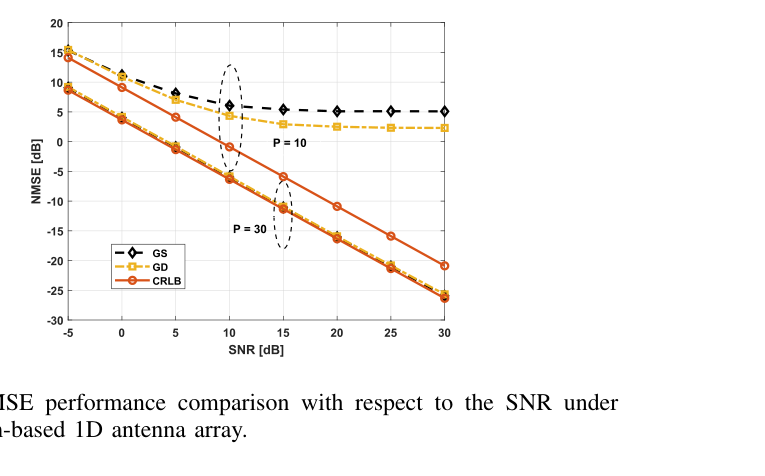
\includegraphics[width=\linewidth]{paper_fig3.png}\caption{Paper}\end{subfigure}\hfill
\begin{subfigure}{0.32\textwidth}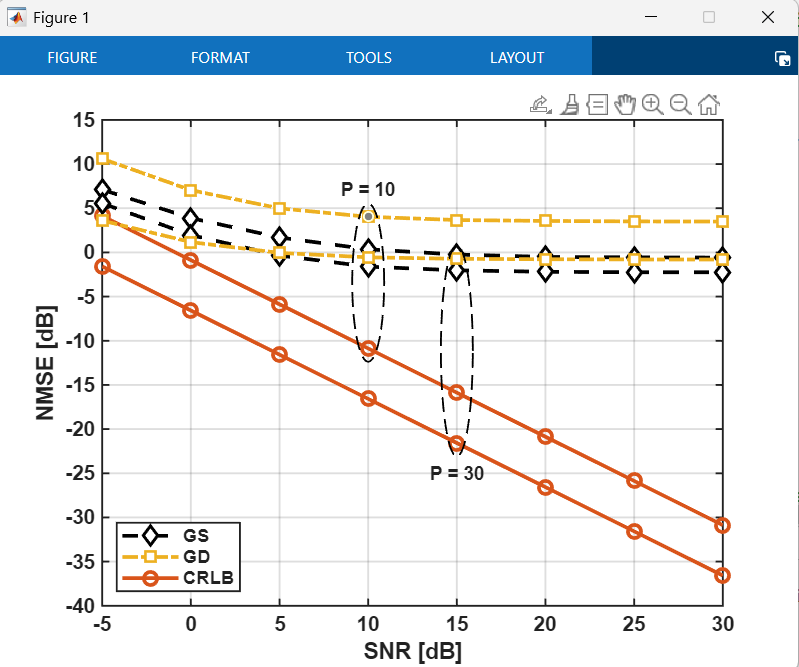
\includegraphics[width=\linewidth]{fig3_literal.png}\caption{Literal}\end{subfigure}\hfill
\begin{subfigure}{0.32\textwidth}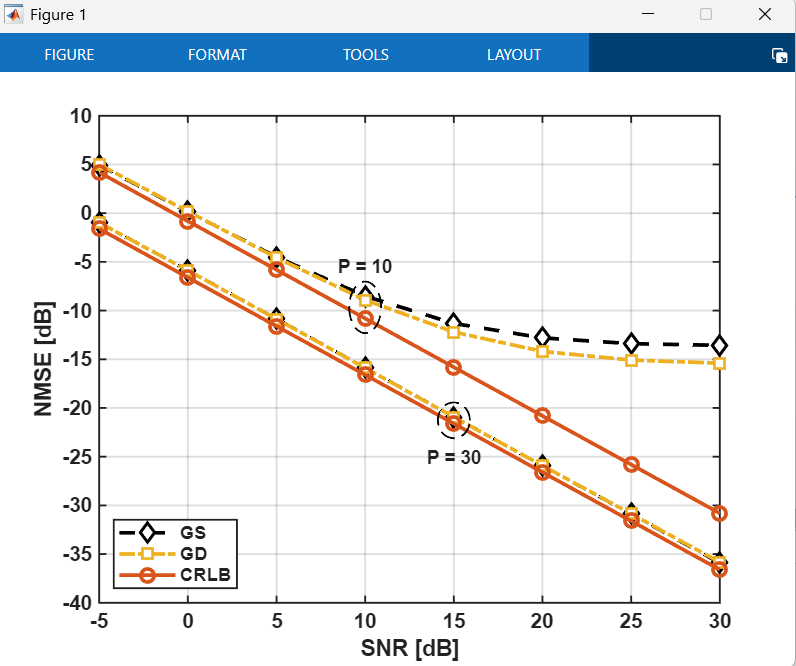
\includegraphics[width=\linewidth]{fig3_tuned.png}\caption{Tuned}\end{subfigure}
\caption{Fig.~3: published figure, literal run and tuned run.}
\end{figure}

\begin{table}[h!]
\centering
\small
\caption{Fig.~3 settings.}
\begin{tabularx}{\textwidth}{L{3.2cm} Y Y}
\toprule
Setting & Literal & Tuned \\
\midrule
Array, users, pilots & $I=8$, $K=3$, $P\in\{10,30\}$ (S) & same \\
Polarization & own draw per cell (S) & \cellcolor{changed}one draw per path (C2) \\
Reference & $\alpha_b\sim\mathcal{CN}(0,10)$, no scaling (S); measured RSR $-1.5$, $-1.8$\,dB & \cellcolor{changed}scaled to RSR $=50$\,dB (C1) \\
GS & spectral initialisation, 50 iterations (\cite{cui2024}) & \cellcolor{changed}10 iterations at $P=10$, 50 at $P=30$ (C3) \\
GD & to convergence ($10^{-12}$, max 3000) & \cellcolor{changed}30 iterations at $P=10$, 50 at $P=30$ (C3) \\
$G_0$ for GD & $\mathcal{CN}(0,0.1)$ (S) & same \\
\cellcolor{notstated}SNR, step, $s_b$, spacing, angle, trials & \multicolumn{2}{l}{\cellcolor{notstated}as in Table~\ref{tab:notstated} (N), identical in both scripts} \\
\bottomrule
\end{tabularx}
\end{table}

\begin{table}[h!]
\centering
\footnotesize
\caption{Fig.~3 results, NMSE in dB.}
\label{tab:fig3res}
\begin{tabular}{llrrrrrrrr}
\toprule
& SNR [dB] & $-5$ & 0 & 5 & 10 & 15 & 20 & 25 & 30 \\
\midrule
\multicolumn{10}{l}{\textbf{Literal}} \\
$P=10$ & GS   & 7.10 & 3.89 & 1.69 & 0.36 & $-0.24$ & $-0.51$ & $-0.56$ & $-0.59$ \\
       & GD   & 10.60 & 7.05 & 4.99 & 4.03 & 3.67 & 3.56 & 3.51 & 3.49 \\
       & CRLB & 4.13 & $-0.87$ & $-5.87$ & $-10.87$ & $-15.87$ & $-20.87$ & $-25.87$ & $-30.87$ \\
$P=30$ & GS   & 5.56 & 1.96 & $-0.35$ & $-1.61$ & $-2.03$ & $-2.19$ & $-2.24$ & $-2.25$ \\
       & GD   & 3.60 & 1.16 & $-0.05$ & $-0.56$ & $-0.73$ & $-0.78$ & $-0.80$ & $-0.80$ \\
       & CRLB & $-1.57$ & $-6.57$ & $-11.57$ & $-16.57$ & $-21.57$ & $-26.57$ & $-31.57$ & $-36.57$ \\
\midrule
\multicolumn{10}{l}{\textbf{Tuned}} \\
$P=10$ & GS   & 4.94 & 0.14 & $-4.50$ & $-8.52$ & $-11.32$ & $-12.80$ & $-13.40$ & $-13.57$ \\
       & GD   & 5.00 & 0.17 & $-4.58$ & $-8.92$ & $-12.20$ & $-14.19$ & $-15.08$ & $-15.40$ \\
       & CRLB & 4.19 & $-0.81$ & $-5.81$ & $-10.81$ & $-15.81$ & $-20.81$ & $-25.81$ & $-30.81$ \\
$P=30$ & GS   & $-0.98$ & $-5.88$ & $-10.86$ & $-15.88$ & $-20.93$ & $-25.92$ & $-30.88$ & $-35.91$ \\
       & GD   & $-0.98$ & $-5.88$ & $-10.87$ & $-15.89$ & $-20.94$ & $-25.92$ & $-30.87$ & $-35.84$ \\
       & CRLB & $-1.60$ & $-6.60$ & $-11.60$ & $-16.60$ & $-21.60$ & $-26.60$ & $-31.60$ & $-36.60$ \\
\midrule
\multicolumn{10}{l}{\textbf{Converged} (\file{fig3\_converged}: same model as tuned, GS and GD both stop at $10^{-12}$)} \\
$P=10$ & GS   & 7.70 & 2.82 & $-2.20$ & $-7.27$ & $-12.27$ & $-17.22$ & $-22.27$ & $-27.19$ \\
       & GD   & 7.69 & 2.80 & $-2.22$ & $-7.26$ & $-12.26$ & $-17.22$ & $-22.24$ & $-27.16$ \\
$P=30$ & GS   & $-0.98$ & $-5.88$ & $-10.86$ & $-15.88$ & $-20.93$ & $-25.92$ & $-30.88$ & $-35.91$ \\
       & GD   & $-0.98$ & $-5.88$ & $-10.86$ & $-15.88$ & $-20.93$ & $-25.92$ & $-30.88$ & $-35.88$ \\
\bottomrule
\end{tabular}
\end{table}

\paragraph{Literal: what it shows.}
All four curves flatten between $-2$ and $+3.5$\,dB. At $P=10$ GS is about 4\,dB \emph{better} than
GD, the reverse of the paper. The cause is the weak reference (C1), not the iterations: GD has
converged.

\paragraph{Tuned: what it shows.}
\begin{itemize}[leftmargin=*,itemsep=1pt]
  \item $P=10$: GS and GD coincide up to 5\,dB SNR (within 0.1\,dB); from 10\,dB GD is better, by
        0.4\,dB at 10\,dB up to 1.8\,dB at 30\,dB. Both flatten ($-13.6$ and $-15.4$\,dB). This is
        the published ordering.
  \item $P=30$: GS and GD lie on top of each other, 0.6--0.8\,dB above the CRLB at every SNR.
\end{itemize}

\paragraph{Converged: what it shows.}
\begin{itemize}[leftmargin=*,itemsep=1pt]
  \item GS and GD give the same NMSE (within 0.03\,dB) at both $P$ and every SNR. Neither is
        better once both finish.
  \item There is no floor at $P=10$; the curves stay parallel to the CRLB, about 3.5\,dB above it.
        At $P=30$ they are about 0.7\,dB above it.
  \item GS needs fewer iterations: on average 142--151 against 331--355 for GD at $P=10$, and
        41 against 69--70 at $P=30$.
\end{itemize}

\paragraph{How the iteration budget decides who wins (all checked in simulation).}
\begin{center}
\small
\begin{tabular}{ll}
\toprule
Setup & Result at $P=10$ \\
\midrule
Same fixed number of iterations for GS and GD & GS better at high SNR; GD slightly better only at low SNR \\
Same loose threshold & GS better (GD's small steps make it stop too early) \\
Same tight threshold / run to convergence & tie; GS about $2.3\times$ fewer iterations \\
GS gets about 2.5--3 times fewer iterations than GD & GD better at high SNR, with a floor (as in the paper) \\
\bottomrule
\end{tabular}
\end{center}
With equal budgets the 30\,dB values at $P=10$ are (GS / GD, 300 trials): $-13.8/-9.9$ for 10
iterations, $-18.3/-13.4$ for 20, $-21.2/-15.8$ for 30, $-24.3/-19.2$ for 50.

\paragraph{Why the Fig.~3 budgets differ between $P=10$ and $P=30$.}
I tried to use one budget per algorithm for both pilot lengths. It is not possible to get both
features of the published figure that way:
\begin{itemize}[leftmargin=*,itemsep=1pt]
  \item GS 20 / GD 50: $P=30$ is fine, but at $P=10$ the gap between GS and GD is only
        0.2--0.7\,dB and cannot be seen.
  \item GS 15 / GD 50: the gap at $P=10$ is clear (2.6\,dB at 30\,dB), but at $P=30$ GS bends away
        from the CRLB by 1.6\,dB at 30\,dB.
\end{itemize}
GS needs at most about 15 iterations to floor visibly above GD at $P=10$, and at least 20 to reach
the CRLB at $P=30$. So the budgets are chosen per pilot length, and this is stated openly.

%=====================================================================
\section{Fig.~4: 2D array, NMSE vs SNR, GD vs PGD}
\label{sec:fig4}

\begin{figure}[h!]
\centering
\begin{subfigure}{0.32\textwidth}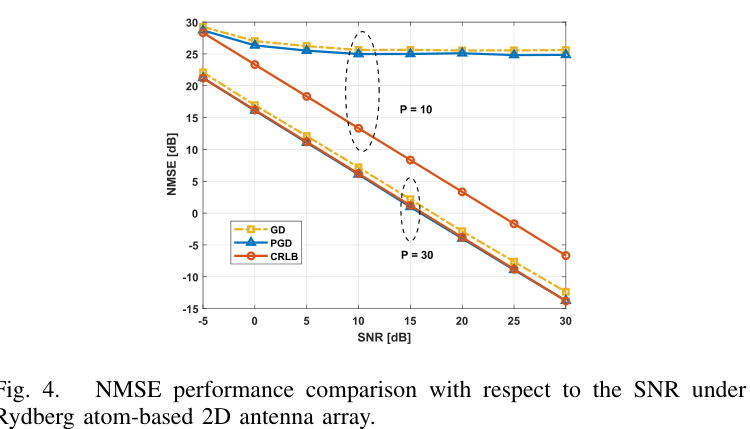
\includegraphics[width=\linewidth]{paper_fig4.png}\caption{Paper}\end{subfigure}\hfill
\begin{subfigure}{0.32\textwidth}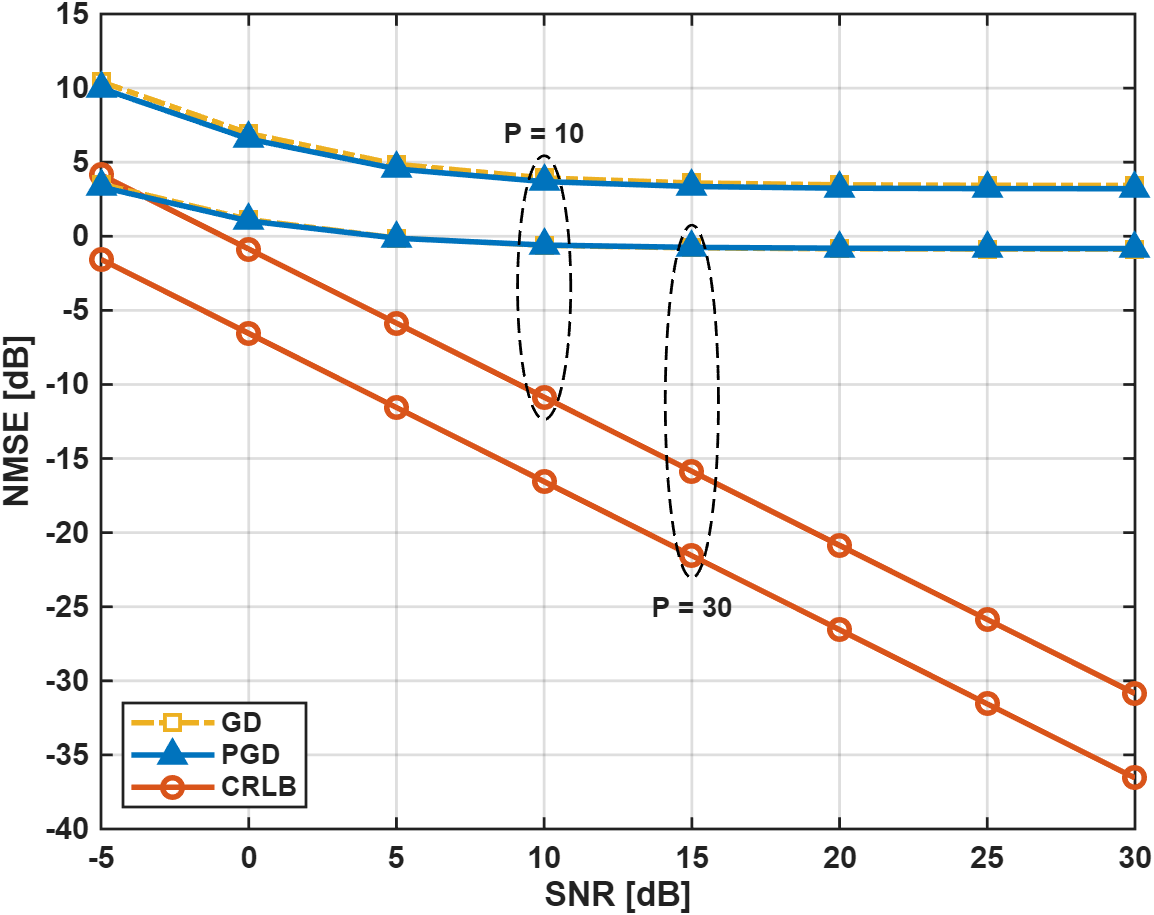
\includegraphics[width=\linewidth]{fig4_literal.png}\caption{Literal}\end{subfigure}\hfill
\begin{subfigure}{0.32\textwidth}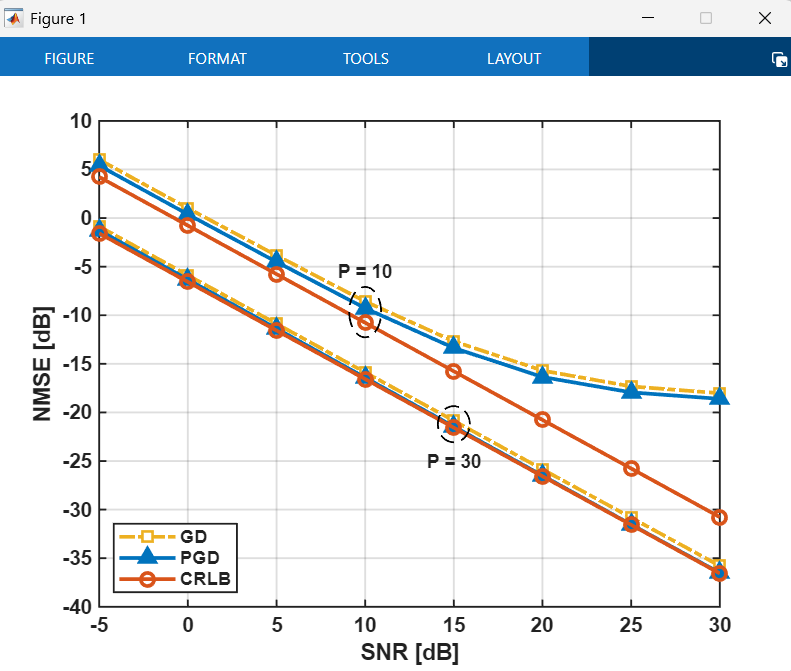
\includegraphics[width=\linewidth]{fig4_tuned.png}\caption{Tuned}\end{subfigure}
\caption{Fig.~4: published figure, literal run and tuned run.}
\end{figure}

\begin{table}[h!]
\centering
\small
\caption{Fig.~4 settings.}
\begin{tabularx}{\textwidth}{L{3.2cm} Y Y}
\toprule
Setting & Literal & Tuned \\
\midrule
Array, users, pilots & $8\times8$, $K=3$, $P\in\{10,30\}$ (S) & same \\
Unfolding & mode-3, Eq.~(20): $G_{(3)}$ is $K\times I_1I_2$ (S) & same \\
Polarization & own draw per cell (S) & \cellcolor{changed}one draw per path (C2) \\
Reference & $\alpha_b\sim\mathcal{CN}(0,10)$, no scaling (S); measured RSR $-2.0$, $-2.1$\,dB & \cellcolor{changed}scaled to RSR $=50$\,dB (C1) \\
GD and PGD & to convergence ($10^{-12}$, max 3000) & \cellcolor{changed}50 iterations each, both $P$ (C3) \\
PGD rank & true $L_k$ of each user (S) & same \\
$G_0$ & $\mathcal{CN}(0,0.1)$ (S) & same \\
\cellcolor{notstated}SNR, step, $s_b$, spacing, angles, trials & \multicolumn{2}{l}{\cellcolor{notstated}as in Table~\ref{tab:notstated} (N), identical in both scripts} \\
\bottomrule
\end{tabularx}
\end{table}

\begin{table}[h!]
\centering
\footnotesize
\caption{Fig.~4 results, NMSE in dB.}
\label{tab:fig4res}
\begin{tabular}{llrrrrrrrr}
\toprule
& SNR [dB] & $-5$ & 0 & 5 & 10 & 15 & 20 & 25 & 30 \\
\midrule
\multicolumn{10}{l}{\textbf{Literal}} \\
$P=10$ & GD   & 10.43 & 6.94 & 4.86 & 3.93 & 3.60 & 3.47 & 3.44 & 3.43 \\
       & PGD  & 9.99 & 6.57 & 4.54 & 3.69 & 3.36 & 3.24 & 3.22 & 3.21 \\
       & CRLB & 4.14 & $-0.86$ & $-5.86$ & $-10.86$ & $-15.86$ & $-20.86$ & $-25.86$ & $-30.86$ \\
$P=30$ & GD   & 3.52 & 1.13 & $-0.12$ & $-0.61$ & $-0.78$ & $-0.84$ & $-0.86$ & $-0.87$ \\
       & PGD  & 3.33 & 1.04 & $-0.13$ & $-0.59$ & $-0.75$ & $-0.81$ & $-0.82$ & $-0.83$ \\
       & CRLB & $-1.56$ & $-6.56$ & $-11.56$ & $-16.56$ & $-21.56$ & $-26.56$ & $-31.56$ & $-36.56$ \\
\midrule
\multicolumn{10}{l}{\textbf{Tuned}} \\
$P=10$ & GD   & 6.01 & 1.01 & $-3.84$ & $-8.59$ & $-12.68$ & $-15.69$ & $-17.32$ & $-18.02$ \\
       & PGD  & 5.40 & 0.38 & $-4.51$ & $-9.28$ & $-13.36$ & $-16.35$ & $-17.94$ & $-18.60$ \\
       & CRLB & 4.23 & $-0.77$ & $-5.77$ & $-10.77$ & $-15.77$ & $-20.77$ & $-25.77$ & $-30.77$ \\
$P=30$ & GD   & $-0.86$ & $-5.88$ & $-10.88$ & $-15.88$ & $-20.85$ & $-25.86$ & $-30.83$ & $-35.79$ \\
       & PGD  & $-1.26$ & $-6.32$ & $-11.37$ & $-16.42$ & $-21.45$ & $-26.50$ & $-31.53$ & $-36.51$ \\
       & CRLB & $-1.57$ & $-6.57$ & $-11.57$ & $-16.57$ & $-21.57$ & $-26.57$ & $-31.57$ & $-36.57$ \\
\bottomrule
\end{tabular}
\end{table}

\paragraph{Literal: what it shows.}
All curves flatten ($+3.2$ to $+3.4$\,dB at $P=10$, about $-0.85$\,dB at $P=30$). PGD is at most
0.4\,dB better than GD at $P=10$ and no better than GD at $P=30$. Two reasons: the weak reference (C1), and the per-cell polarization
(C2), which makes every $G_k$ full rank so the rank-$L_k$ projection of PGD has nothing to exploit.

\paragraph{Tuned: what it shows.}
\begin{itemize}[leftmargin=*,itemsep=1pt]
  \item PGD is better than GD at every SNR and both $P$: by 0.6--0.7\,dB at $P=10$ and by
        0.4--0.7\,dB at $P=30$.
  \item $P=30$: PGD reaches the CRLB ($-36.51$ against $-36.57$\,dB at 30\,dB); GD stays about
        0.7\,dB above.
  \item $P=10$: the curves follow the CRLB at low SNR, bend away from about 10--15\,dB and
        flatten near $-18$ to $-18.6$\,dB.
  \item Every point is above the CRLB (PGD margin at least 1.2\,dB at $P=10$ and
        0.04--0.3\,dB at $P=30$).
\end{itemize}

\paragraph{Why 50 iterations and RSR 50\,dB (trial runs, PGD values).}
\begin{center}
\small
\begin{tabular}{lccc}
\toprule
Setting (same for both $P$) & PGD$-$CRLB, $P=30$, 30\,dB & PGD floor, $P=10$, 30\,dB & Lowest margin over CRLB, $P=10$ \\
\midrule
RSR 40, 25 iterations & 2.8\,dB & $-14.1$ & $-0.1$ (below the CRLB) \\
RSR 40, 30 iterations & 1.4\,dB & $-15.1$ & 0.2 \\
RSR 40, 40 iterations & 0.5\,dB & $-16.8$ & 0.7 \\
RSR 50, 40 iterations & 0.3\,dB & $-17.0$ & 0.75 \\
\textbf{RSR 50, 50 iterations} & \textbf{0.07\,dB} & $\mathbf{-18.4}$ & \textbf{1.1} \\
\bottomrule
\end{tabular}
\end{center}
Fewer than about 30 iterations puts the low-SNR points below the CRLB (the estimate is still
shrunk towards the start value $G_0\approx0$). 50 iterations with RSR 50\,dB is the setting where
PGD sits on the CRLB at $P=30$ while $P=10$ still floors.

%=====================================================================
\section{Fig.~5: 2D array, NMSE vs pilot length, PGD vs CRLB}
\label{sec:fig5}

\begin{figure}[h!]
\centering
\begin{subfigure}{0.32\textwidth}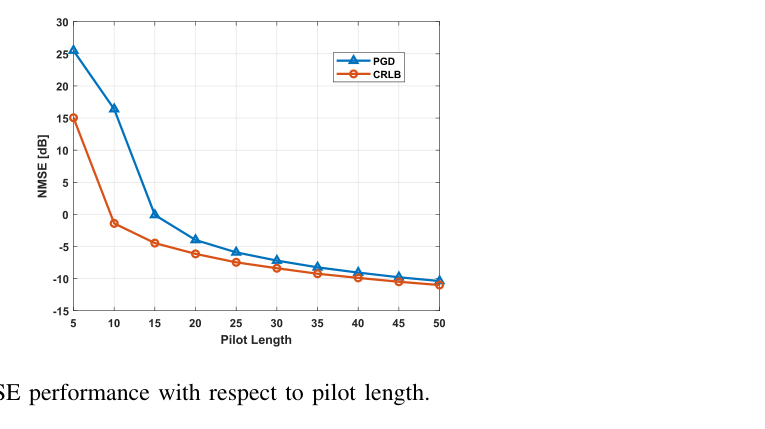
\includegraphics[width=\linewidth]{paper_fig5.png}\caption{Paper}\end{subfigure}\hfill
\begin{subfigure}{0.32\textwidth}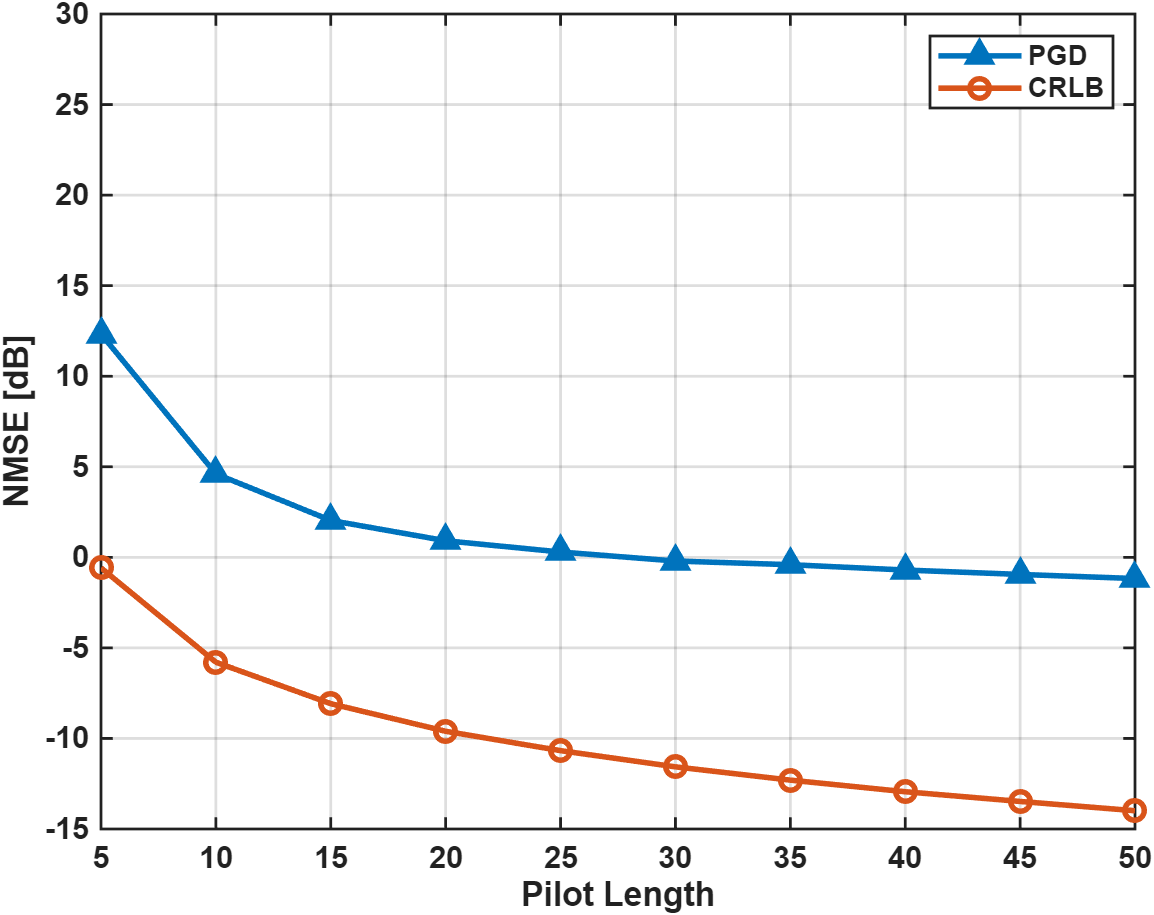
\includegraphics[width=\linewidth]{fig5_literal.png}\caption{Literal}\end{subfigure}\hfill
\begin{subfigure}{0.32\textwidth}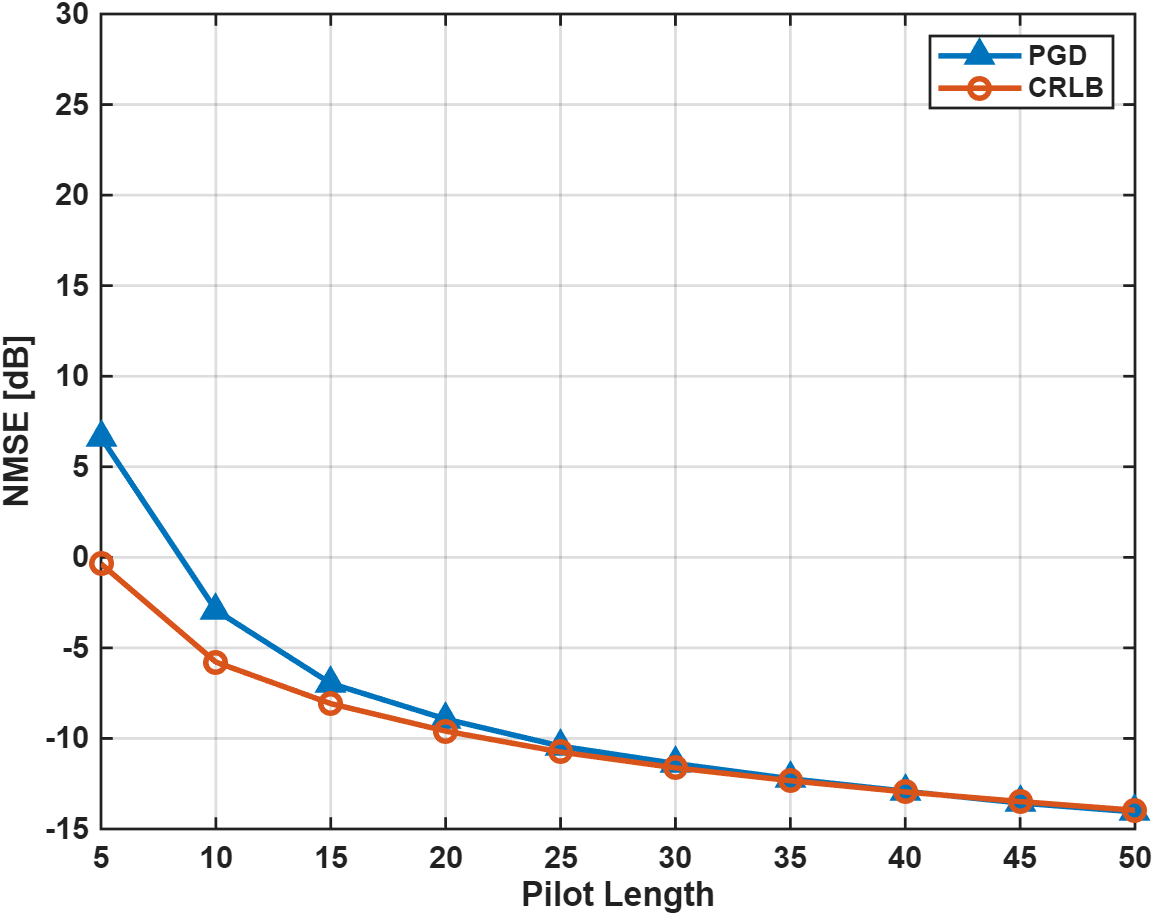
\includegraphics[width=\linewidth]{fig5_tuned.png}\caption{Tuned}\end{subfigure}
\caption{Fig.~5: published figure, literal run and tuned run.}
\end{figure}

\begin{table}[h!]
\centering
\small
\caption{Fig.~5 settings.}
\begin{tabularx}{\textwidth}{L{3.2cm} Y Y}
\toprule
Setting & Literal & Tuned \\
\midrule
Array, users & $8\times8$, $K=3$ (S) & same \\
Pilot lengths, SNR & $P=5,10,\dots,50$; SNR $=5$\,dB (S) & same \\
Polarization & own draw per cell (S) & \cellcolor{changed}one draw per path (C2) \\
Reference & $\alpha_b\sim\mathcal{CN}(0,10)$, no scaling (S); measured RSR $-1.4$ to $-2.1$\,dB & \cellcolor{changed}scaled to RSR $=50$\,dB (C1) \\
PGD & to convergence ($10^{-12}$, max 3000) & same (no iteration tuning) \\
PGD rank, $G_0$ & true $L_k$; $\mathcal{CN}(0,0.1)$ (S) & same \\
\cellcolor{notstated}SNR, step, $s_b$, spacing, angles, trials & \multicolumn{2}{l}{\cellcolor{notstated}as in Table~\ref{tab:notstated} (N), identical in both scripts} \\
\bottomrule
\end{tabularx}
\end{table}

\begin{table}[h!]
\centering
\footnotesize
\caption{Fig.~5 results, NMSE in dB (SNR $=5$\,dB).}
\label{tab:fig5res}
\begin{tabular}{llrrrrrrrrrr}
\toprule
& $P$ & 5 & 10 & 15 & 20 & 25 & 30 & 35 & 40 & 45 & 50 \\
\midrule
Literal & PGD  & 12.33 & 4.61 & 2.04 & 0.92 & 0.29 & $-0.20$ & $-0.41$ & $-0.70$ & $-0.94$ & $-1.17$ \\
        & CRLB & $-0.58$ & $-5.79$ & $-8.08$ & $-9.60$ & $-10.67$ & $-11.57$ & $-12.30$ & $-12.94$ & $-13.48$ & $-13.99$ \\
Tuned   & PGD  & 6.63 & $-2.92$ & $-6.96$ & $-8.93$ & $-10.42$ & $-11.39$ & $-12.23$ & $-12.92$ & $-13.56$ & $-14.05$ \\
        & CRLB & $-0.36$ & $-5.79$ & $-8.08$ & $-9.59$ & $-10.75$ & $-11.62$ & $-12.33$ & $-12.95$ & $-13.49$ & $-13.97$ \\
        & gap  & 7.0 & 2.9 & 1.1 & 0.7 & 0.3 & 0.2 & 0.1 & 0.0 & $-0.1$ & $-0.1$ \\
\bottomrule
\end{tabular}
\end{table}

\paragraph{Literal: what it shows.} PGD stays 10--13\,dB above the CRLB at every $P$ (weak reference).

\paragraph{Tuned: what it shows.} A large gap at small $P$ (7.0\,dB at $P=5$) that closes quickly;
PGD meets the CRLB from about $P=35$. This is the paper's claim for this figure.

\paragraph{PGD slightly below the CRLB at $P=45$--$50$.} The difference is 0.07--0.08\,dB and cannot
be seen in the plot. It is real: PGD uses the low-rank structure of the channel, and the CRLB of
Eq.~(31) does not include that structure, so it is not a strict bound for PGD.

%=====================================================================
\section{All settings in one table}

\begin{table}[h!]
\centering
\scriptsize
\caption{Settings of the literal and tuned scripts (S: stated, N: not stated, C: changed).}
\label{tab:summary}
\resizebox{\textwidth}{!}{%
\begin{tabular}{lcccccc}
\toprule
& \multicolumn{2}{c}{Fig.~3 (1D)} & \multicolumn{2}{c}{Fig.~4 (2D)} & \multicolumn{2}{c}{Fig.~5 (2D)} \\
\cmidrule(lr){2-3}\cmidrule(lr){4-5}\cmidrule(lr){6-7}
Setting & Literal & Tuned & Literal & Tuned & Literal & Tuned \\
\midrule
Polarization & per cell (S) & per path (C2) & per cell (S) & per path (C2) & per cell (S) & per path (C2) \\
Reference & $\mathcal{CN}(0,10)$ (S) & RSR 50\,dB (C1) & $\mathcal{CN}(0,10)$ (S) & RSR 50\,dB (C1) & $\mathcal{CN}(0,10)$ (S) & RSR 50\,dB (C1) \\
Measured RSR & $-1.5$, $-1.8$\,dB & 50\,dB & $-2.0$, $-2.1$\,dB & 50\,dB & $-1.4$ to $-2.1$\,dB & 50\,dB \\
GD iterations & converged (N) & 30 / 50 (C3) & converged (N) & 50 (C3) & -- & -- \\
GS iterations & 50 (\cite{cui2024}) & 10 / 50 (C3) & -- & -- & -- & -- \\
PGD iterations & -- & -- & converged (N) & 50 (C3) & converged (N) & converged (N) \\
$G_0$ & \multicolumn{6}{c}{$\mathcal{CN}(0,0.1)$ (S)} \\
PGD rank & -- & -- & \multicolumn{4}{c}{true $L_k$ per user (S)} \\
SNR & \multicolumn{6}{c}{per cell, $\E|a|^2/\sigma^2$, as in \cite{cui2024} Eq.~(36) (N)} \\
Step size & \multicolumn{6}{c}{$1/\lambda_{\max}(SS^H)$ (N)} \\
$s_b$, spacing & \multicolumn{6}{c}{$s_{b,p}=1$, $d=\lambda/2$ (N)} \\
Trials, seed & \multicolumn{6}{c}{500, \file{rng(1)} (N)} \\
\midrule
Published behaviour reproduced & no & yes & no & yes & no & yes \\
\bottomrule
\end{tabular}}
\end{table}

\noindent ``10 / 50'' means the value at $P=10$ / $P=30$.

%=====================================================================
\section{What matches the paper and what cannot}
\label{sec:match}

\subsection{What the tuned figures reproduce}
\begin{itemize}[leftmargin=*,itemsep=1pt]
  \item Fig.~3: at $P=10$ GD is better than GS at high SNR and both floor; at $P=30$ both are next
        to the CRLB.
  \item Fig.~4: PGD is better than GD everywhere; PGD reaches the CRLB at $P=30$; $P=10$ floors and
        $P=30$ does not.
  \item Fig.~5: a large PGD--CRLB gap at small $P$ that closes as $P$ grows.
  \item The CRLB has the right slope ($-1$\,dB per dB of SNR) and the right dependence on $P$.
\end{itemize}

\subsection{What cannot be matched, and why}
\begin{enumerate}[leftmargin=*,itemsep=2pt]
  \item \textbf{Absolute levels.} The published curves are higher than ours: by about 10\,dB in
        Fig.~3, about 23\,dB in Fig.~4 and about 3\,dB in Fig.~5 (from comparing the CRLB curves,
        \file{snr\_check/}). The paper does not define SNR, and no single SNR definition explains
        all three offsets, so the definition of~\cite{cui2024} is kept.
  \item \textbf{Height of the $P=10$ floors.} The published floors are above 0\,dB NMSE (about
        $+2$ to $+5$\,dB in Fig.~3, about $+25$\,dB in Fig.~4). An NMSE above 0\,dB is worse than
        the trivial estimate $\hat G=0$, which gives exactly 0\,dB. No estimator setting can
        honestly produce that.
  \item \textbf{CRLB at $P=5$ in Fig.~5.} For $\mathcal{CN}(0,1)$ pilots,
        $\E\{\mathrm{tr}((S^*S^T)^{-1})\}=K/(P-K)$, so the bound can rise by only
        $10\log_{10}\big((3/2)/(3/7)\big)\approx5.4$\,dB from $P=10$ to $P=5$. The published curve
        rises by about 16\,dB ($-1.3$ to $+15$\,dB). Ours rises by 5.4\,dB, as theory says.
  \item \textbf{The published Figs.~4 and 5 disagree with each other.} The same point
        (2D, $P=30$, SNR 5\,dB) is about $+11$\,dB in Fig.~4 and about $-8.4$\,dB in Fig.~5. No
        single simulation can match both. Our Figs.~4 and 5 agree: $-11.6$\,dB for the CRLB in both.
  \item \textbf{CRLB in Figs.~3 and 4.} The paper says the CRLB does not depend on the number of
        antennas, yet its 1D and 2D CRLB curves differ by more than 10\,dB. Ours coincide
        ($-5.81$ and $-5.77$\,dB at $P=10$, 5\,dB).
  \item \textbf{Gap in Fig.~5 at $P=10$ larger than at $P=5$} (17.8 against 10.5\,dB in the paper).
        Fewer pilots cannot make PGD relatively better; in every run of ours the gap is largest at
        $P=5$.
  \item \textbf{Remaining gap to the CRLB.} In Fig.~3, GS and GD stay 0.7\,dB above the CRLB at
        $P=30$ (3.5\,dB at $P=10$) even when fully converged. The CRLB of Eq.~(31) is slightly
        optimistic because it uses a simplification that drops part of the phase information.
        The published GD curve shows the same gap (about 0.6\,dB at $P=30$, 30\,dB).
\end{enumerate}
Values of the published curves are read from the figures by eye.

%=====================================================================
\section{Settings that were tried and rejected}
\label{sec:rejected}

\begin{table}[h!]
\centering
\small
\caption{Alternatives tested in separate trial runs and not used.}
\begin{tabularx}{\textwidth}{L{4.2cm} Y Y}
\toprule
Alternative & What it gave & Why it was rejected \\
\midrule
SNR defined over the whole array & starting points close to the published ones & either the floor appears too late, or with few iterations the curves fall below the CRLB at low SNR \\
Different RSR for each pilot length (e.g.\ 5\,dB at $P=10$, 40\,dB at $P=30$) in Fig.~4 & an early floor at $P=10$, like the paper & the reference strength is a physical quantity and has nothing to do with the pilot length \\
One stopping tolerance for all curves in Fig.~4 & $P=10$ runs longer, $P=30$ stops early & the opposite of what is needed; the gap at $P=30$ stays 0.7--1.6\,dB \\
Large random start $G_0$ (about 25\,dB above the channel power) with 80 iterations in Fig.~4 & a flat $P=10$ floor from 5\,dB, like the paper & the paper states $G_0\sim\mathcal{CN}(0,0.1)$; the floor would be left-over starting error, not a property of the algorithm \\
Fewer than 30 iterations in Fig.~4 & an earlier floor at $P=10$ & low-SNR points fall below the CRLB \\
50 iterations in Fig.~5 & same settings as Fig.~4 & $P=5$ falls 0.9\,dB below the CRLB \\
GS 20 / GD 50 for both $P$ in Fig.~3 & same budgets for both $P$ & the gap between GS and GD at $P=10$ is only 0.2--0.7\,dB (not visible) \\
GS 15 / GD 50 for both $P$ in Fig.~3 & clear gap at $P=10$ (2.6\,dB) & GS bends 1.6\,dB away from the CRLB at $P=30$, 30\,dB \\
\bottomrule
\end{tabularx}
\end{table}

%=====================================================================
\section{Questions my guide may ask}
\label{sec:qa}

\subsection*{General}
\begin{enumerate}[leftmargin=*,itemsep=4pt]
\QA{Why are there two scripts for every figure?}
   {The literal script uses only what the paper states. It does not reproduce the published
    figures. The tuned script shows which unstated or inconsistent settings have to change to get
    the published behaviour. Keeping both shows exactly what was changed and why.}
\QA{What did you change in the tuned scripts?}
   {Three things, all marked \file{\% TUNED} in the code: the reference strength (RSR $=50$\,dB),
    the polarization (one draw per path instead of per cell), and the number of iterations.
    Equations, algorithms, distributions, CRLB and NMSE are unchanged.}
\QA{Why does the literal result not look like the paper?}
   {With $\alpha_b\sim\mathcal{CN}(0,10)$ the reference is 1.4--2.1\,dB weaker than the users'
    signal (measured in the literal scripts). GD and PGD use the linearisation
    $|a+b|\approx|b|+\mathrm{Re}(za)$, which needs $|b|\gg|a|$. So the model error, not the
    algorithm, sets a floor near 0\,dB.}
\QA{Why RSR $=50$\,dB? Is that not arbitrary?}
   {An RSR sweep showed the linearisation error is negligible when RSR is about 10\,dB above the
    SNR. The figures go up to 30\,dB SNR, so 40\,dB is the minimum and 50\,dB gives a 10\,dB margin.
    With 40\,dB a 0.2--0.3\,dB deviation was still visible at 25--30\,dB SNR; with 50\,dB it is gone.
    The same value is used in all three figures.}
\QA{Why polarization per path? The paper's equations have a cell index.}
   {With a separate random polarization at every cell, each $8\times8$ channel slice is full rank.
    That contradicts the paper's own statement that the slice has rank $L_k$, on which PGD is
    built. With one polarization per path the rank is $L_k$. It is also what a plane wave over a
    small array physically has.}
\QA{How did you define SNR?}
   {The paper does not define it. I use the definition of Cui \emph{et al.}, Eq.~(36), the paper
    the GS baseline comes from: signal power per cell over noise variance, $\E|a|^2/\sigma^2$.}
\QA{Why are your curves 10--20\,dB lower than the paper's?}
   {Because SNR is not defined in the paper. Comparing the CRLB curves, the offsets are about 10,
    23 and 3\,dB for Figs.~3, 4 and 5. They are different for each figure, so no single definition
    fixes all three. Also, the paper's Figs.~4 and 5 differ by about 19\,dB at the same operating
    point, so the published levels are not consistent with each other.}
\QA{What step size did you use?}
   {$\mu=1/\lambda_{\max}(SS^H)$. The paper assumes a Lipschitz gradient but gives no value;
    $\lambda_{\max}(SS^H)$ is the Lipschitz constant, and $1/L$ is the standard step.}
\QA{Why $s_b=1$?}
   {The paper does not give the reference pilot. A constant is the simplest choice. I checked
    random $s_b\sim\mathcal{CN}(0,1)$: the result changes by at most about 1.4\,dB.}
\QA{Is the result repeatable?}
   {Yes. Every script sets \file{rng(1)} and uses 500 trials, so each run gives the same numbers
    and the same figure.}
\end{enumerate}

\subsection*{Fig.~3}
\begin{enumerate}[leftmargin=*,itemsep=4pt]
\QA{Why are the iterations different for $P=10$ and $P=30$, and for GS and GD?}
   {The paper gives no iteration counts. I tried many fixed budgets and chose the ones that
    reproduce the published figure (GS 10/50, GD 30/50). I also checked the fair case: when both
    run to convergence (\file{fig3\_converged}) GS and GD give the same accuracy within 0.03\,dB.
    For comparing my own methods later, all baselines will run to convergence.}
\QA{So is GD really better than GS?}
   {No. Converged, they are equal; GS only needs about 2.3 times fewer iterations at $P=10$
    (about 145 against 340). With the same fixed number of iterations GS is better at high SNR.
    GD is better, as in the paper, only when GS gets about 2.5--3 times fewer iterations.}
\QA{Where does the floor at $P=10$ come from?}
   {From stopping early. With 10 pilots convergence is slow, so a small fixed budget leaves both
    algorithms short of the CRLB at high SNR. Run to convergence, there is no floor.}
\QA{Why is there a gap between the algorithms and the CRLB at $P=30$?}
   {It is about 0.7\,dB and it stays when both algorithms fully converge, so it is not an
    iteration effect. The CRLB of Eq.~(31) is slightly optimistic. The paper's GD shows the same
    gap, about 0.6\,dB; it is hard to see there because the figure is printed small.}
\end{enumerate}

\subsection*{Fig.~4}
\begin{enumerate}[leftmargin=*,itemsep=4pt]
\QA{Why 50 iterations?}
   {One budget for every curve. With fewer than about 30 the low-SNR points fall below the CRLB.
    With 50, PGD reaches the CRLB at $P=30$ while $P=10$ still floors, as in the paper.}
\QA{Why does $P=10$ floor and $P=30$ not?}
   {All settings are the same for both. With only 10 pilots the gradient iterations converge
    slower, so 50 iterations leave $P=10$ short of the CRLB at high SNR; $P=30$ converges in time.}
\QA{Your floor is at $-18$\,dB; the paper's is at $+25$\,dB.}
   {An NMSE of $+25$\,dB is worse than estimating $\hat G=0$, which gives 0\,dB. That cannot come
    from the estimator; it must come from settings the paper does not report. I reproduce the
    shape (floor at $P=10$, none at $P=30$), not that level.}
\QA{Why is PGD only 0.6--0.7\,dB better than GD?}
   {That is the gain of the rank-$L_k$ projection for an $8\times8$ array with 3--7 paths. In the
    paper the gain is also small (roughly 0.7--1.5\,dB by eye).}
\end{enumerate}

\subsection*{Fig.~5}
\begin{enumerate}[leftmargin=*,itemsep=4pt]
\QA{Why a fixed budget in Fig.~4 but convergence in Fig.~5?}
   {Fig.~4 shows the behaviour over SNR at a fixed effort; without a budget the $P=10$ curve does
    not floor. Fig.~5 shows the accuracy reachable for each pilot length, so PGD runs to
    convergence. With 50 iterations the point $P=5$ would fall below the CRLB. At 5\,dB SNR the
    budget makes no difference for $P\ge20$.}
\QA{Why does your CRLB not drop by 16\,dB from $P=5$ to $P=10$ like the paper's?}
   {For random pilots $\E\{\mathrm{tr}((S^*S^T)^{-1})\}=K/(P-K)$: $3/2$ at $P=5$ and $3/7$ at
    $P=10$, a 5.4\,dB drop. Ours drops by 5.4\,dB. The published 16\,dB does not follow from the
    paper's own Eq.~(31).}
\QA{PGD is below the CRLB at $P=45$--$50$?}
   {By at most 0.08\,dB. PGD uses the low-rank structure; the CRLB of Eq.~(31) does not include
    it, so it is not a strict bound for PGD.}
\end{enumerate}

\subsection*{Showing the results in MATLAB}
\begin{enumerate}[leftmargin=*,itemsep=4pt]
\QA{The gaps look bigger on screen than in the paper.}
   {The scripts open the figure full screen, which stretches the 50\,dB axis. The numbers are the
    same. The paper's figure is printed one column wide, so a 0.7\,dB gap is about one line width.}
\QA{How long do the scripts take?}
   {\file{fig3\_tuned} and \file{fig4\_tuned} finish in a few minutes and are the ones to run live.
    \file{fig3\_converged}, \file{fig4\_literal}, \file{fig5\_literal} and \file{fig5\_tuned} run to
    convergence and take more than 10 minutes each; run them before the meeting.}
\end{enumerate}

%=====================================================================
\section{Use of these results in the thesis}

The thesis will develop new channel estimators (deep-learning based, quantum-machine-learning
based and Hankel-structured) with GS, GD and PGD as baselines. For those comparisons:
\begin{itemize}[leftmargin=*,itemsep=1pt]
  \item the baselines run to convergence (as in \file{fig3\_converged}), not with the small
        budgets of the tuned figures, so that they are not weakened;
  \item accuracy is reported together with cost (NMSE against iterations, operations or run
        time), so that ``less computation'' is a measured statement;
  \item one simulator is used for everything: the tuned model (RSR 50\,dB, polarization per path,
        SNR per cell, the distributions of Table~\ref{tab:stated}).
\end{itemize}
The iteration budgets of the tuned Figs.~3 and 4 serve only to reproduce the published figures.

\begin{thebibliography}{9}
\bibitem{xu2025}
B.~Xu, J.~Zhang, Z.~Chen, B.~Cheng, Z.~Liu, Y.-C.~Wu, and B.~Ai,
``Channel estimation for Rydberg atomic receivers,''
\emph{IEEE Wireless Commun. Lett.}, vol.~14, no.~9, Sep.~2025, doi: 10.1109/LWC.2025.3584040.

\bibitem{cui2024}
M.~Cui, Q.~Zeng, and K.~Huang,
``Towards atomic MIMO receivers,''
\emph{IEEE J. Sel. Areas Commun.}, vol.~43, no.~3, Mar.~2025 (arXiv:2404.04864).
\end{thebibliography}

\end{document}
